%!TeX program = xelatex
\documentclass[12pt,hyperref,a4paper,UTF8]{ctexart}
\usepackage{zjureport}
\usepackage{listings}
\usepackage{enumitem}
\usepackage{float}
\usepackage{xcolor}
\lstset{
    %backgroundcolor=\color{red!50!green!50!blue!50},%代码块背景色为浅灰色
    rulesepcolor= \color{gray}, %代码块边框颜色
    breaklines=true,  %代码过长则换行
    numbers=left, %行号在左侧显示
    numberstyle= \small,%行号字体
    keywordstyle= \color{blue},%关键字颜色
    commentstyle=\color{gray}, %注释颜色
    frame=shadowbox%用方框框住代码块
    basicstyle=\small\ttfamily % 设置代码块的基本字体样式
    }


%%-------------------------------正文开始---------------------------%%
\begin{document}

%%-----------------------封面--------------------%%
\cover


\thispagestyle{empty} % 首页不显示页码
\newpage


%%------------------摘要-------------%%
\begin{abstract}
本文深入研究了基于超表面的光谱重建技术，
从超表面设计、光谱重建算法到实验分析进行了全面探讨。
首先，设计并仿真了25组不同响应函数的超表面，通过调整光栅参数实现了对不同波长光的高效调控。
其次，采用基于高斯基展开的正则化方法进行光谱重建，
该方法通过将光谱信号表示为高斯基函数的线性组合，
并利用Tikhonov正则化抑制噪声，实现了从压缩信号到光谱分布的有效重建。
实验部分系统分析了采样间隔、光谱特征宽度以及噪声强度等因素对重建效果的影响，
结果表明我们的光谱重建性能为：单峰光谱的分辨率极限约为6nm，双峰光谱的分辨率极限约为40nm，抗噪声极限约为0.7。
研究还指出，宽光谱因频率成分复杂且响应函数数量有限，重建效果不佳。
本研究验证了基于超表面的光谱重建技术的可行性，同时也揭示了其性能边界，
为未来优化超表面设计和改进重建算法提供了重要参考，展示了该技术在生物医学、
环境监测等领域的应用潜力。
\end{abstract}

%%------------------关键词-------------%%
\begin{flushleft}
\textbf{关键词：} 超表面, 光谱重建, 高斯基展开, 正则化方法, 光电流, 光谱重构算法, 抗噪声性能
\end{flushleft}


%%--------------------------目录页------------------------%%
\newpage
\tableofcontents

%%------------------------正文页从这里开始-------------------%
\newpage

%%可选择这里也放一个标题
%\begin{center}
%    \title{ \Huge \textbf{{标题}}}
%\end{center}


% \keywords{}

\section{背景}
\subsection{超表面的基本概念与特性}
超表面（Metasurface）是一种由亚波长尺度人工微结构（“元原子”，meta-atoms）组成的二维平面材料。通过精心设计这些微结构的几何形状、尺寸和排列方式，超表面能够对电磁波的振幅、相位、偏振以及光谱特性进行灵活调控。与传统的体光学元件（如透镜和棱镜）相比，超表面具有以下显著优势：
\begin{itemize}
    \item \textbf{超薄性}：超表面的厚度通常在亚波长尺度范围内，远小于传统光学元件的尺寸。
    \item \textbf{低损耗}：通过优化材料和结构设计，超表面能够在宽光谱范围内实现高效的光学调控。
    \item \textbf{易集成性}：超表面可以直接集成到芯片或其他微型光学系统中，适用于便携化和高集成度的应用场景。
    \item \textbf{功能多样性}：通过设计不同的微结构，超表面能够实现传统光学元件难以实现的功能，例如同时调控光的相位和偏振。
\end{itemize}

\begin{figure}[H]
\centering

\includegraphics[width=0.8\textwidth]{figures/fig/image1.png}
\caption{超表面的示意图\cite{neshev2018optical}}
\end{figure}

近年来，超表面在光谱成像领域的研究取得了突破性进展，其核心能力主要体现在以下两个方面：
\begin{enumerate}
    \item \textbf{多维光场调控}：超表面通过引入色散调控的琼斯矩阵设计，可以在波长维度上扩展偏振调控自由度，从而实现光谱-偏振的联合重构。这种能力使得超表面能够在单一器件中同时实现多种光学功能。
    \item \textbf{压缩感知采样}：超表面可以被设计为物理层的压缩编码器，其每个“超像素”（superpixel）包含数千个手性元原子阵列，能够对入射光的光谱和偏振信息进行高效编码。这种设计显著提高了光谱信息的采集效率。
\end{enumerate}

超表面的这些特性使其成为光谱成像和信息处理领域的重要研究方向，为传统光学系统的革新提供了新的可能性。

\subsection{散斑光谱仪的工作原理}
传统光谱仪通常依赖色散元件（如光栅）或滤光片分离不同波长的光谱信号，这种方法虽然成熟，但由于需要复杂的光学系统，导致设备体积庞大、成本较高且成像速度受限。
而散斑光谱仪通过一种颠覆性的架构设计，克服了这些限制，展现出紧凑化、高效化和多功能化的优势。

\begin{figure}[H]
\centering

\includegraphics[width=0.8\textwidth]{figures/fig/image2.png}
\caption{散斑光谱仪的工作原理示意图\cite{wan2021review}}
\end{figure}

基于超表面的散斑光谱仪的工作原理主要包括以下几个关键步骤：

\begin{itemize}
    \item \textbf{光谱编码机制}：当入射光谱通过超表面时，超表面利用其精心设计的亚波长微结构对光波进行调制。具体而言，超表面通过改变微结构的几何形状、排列方式和材料特性，能够对不同波长的光进行选择性透射或反射。准随机超级单元（quasi-random supercells）的设计进一步提升了光谱调控的自由度，使得超表面能够同时覆盖窄带和宽带光谱信号。这种编码机制将光谱信息映射为空间或强度上的特定分布，为后续的信号处理提供了基础。

    \item \textbf{光电流转换}：经过超表面调制的光信号被传输到图像传感器（如CMOS或CCD），并在传感器中被转换为电信号。此过程的关键在于超表面与传感器的协同设计。例如，单晶硅超表面可以直接集成到CMOS芯片上，在可见光波段（400--800 nm）实现高效的光电转换。即使光学系统的F数在较大范围内变化（如从F/1.8到F/8），超表面仍能保持较高的光谱重构精度。这种高孔径鲁棒性使得超表面光谱仪在复杂光学环境下依然能够稳定工作。

    \item \textbf{信号采集与压缩感知}：由于超表面光谱仪的设计目标是实现紧凑化和高效化，其传感器通常不会直接采集完整的光谱信息，而是获取经过超表面编码后的压缩信号。通过合理设计超表面的微结构，可以构建出具有稀疏特性的测量矩阵，从而满足压缩感知理论的要求。这种方法不仅减少了数据采集量，还显著提高了系统的采样效率。

    \item \textbf{光谱重构}：传感器采集到的压缩信号需通过数学算法重构出原始光谱信息。重构过程通常基于以下数学模型：
    \[
    \mathbf{y} = \mathbf{\Phi} \mathbf{\Psi} \mathbf{x} + \mathbf{e}
    \]
    其中，\(\mathbf{x}\)为原始光谱，\(\mathbf{\Phi}\)为超表面构建的测量矩阵，\(\mathbf{\Psi}\)为稀疏基矩阵（如小波基），\(\mathbf{y}\)为观测信号，\(\mathbf{e}\)为噪声。通过求解该模型，可以从有限的观测信号中重构出高分辨率的光谱。常用的重构算法包括正交匹配追踪（OMP）、分段自适应采样优化（SASCS）以及基于深度学习的卷积神经网络方法。这些算法能够在不同场景下平衡重构精度与计算效率。

\end{itemize}

综上所述，超表面光谱仪通过将光谱编码、光电转换和压缩感知相结合，显著简化了传统光谱仪的光学系统，同时提升了光谱测量的效率和灵活性。这种新型光谱仪在生物医学、环境监测和工业检测等领域展现出广阔的应用前景。

\subsection{光谱重构算法}
光谱重构算法的目标是从传感器采集的压缩信号中重建原始光谱信息。基于超表面的光谱仪通过对入射光谱进行编码，将光谱信息压缩为有限的观测信号。通常采用以下数学模型描述这一过程：
\[
\mathbf{y} = \mathbf{\Phi} \mathbf{\Psi} \mathbf{x} + \mathbf{e}
\]
其中：
\begin{itemize}
    \item \(\mathbf{x}\)：原始光谱信号；
    \item \(\mathbf{\Phi}\)：测量矩阵，由超表面的编码特性决定；
    \item \(\mathbf{\Psi}\)：稀疏基矩阵（如小波基或傅里叶基）；
    \item \(\mathbf{y}\)：传感器采集的压缩信号；
    \item \(\mathbf{e}\)：噪声项。
\end{itemize}

\begin{figure}[H]
\centering

\includegraphics[width=0.8\textwidth]{figures/fig/image3.png}
\caption{光谱重构算法示意图\cite{qilin2021research}}
\end{figure}


为了解决这一逆问题，常用的光谱重构算法包括：
\begin{enumerate}
    \item \textbf{正交匹配追踪（OMP）}：通过迭代选择最相关的基向量，逐步逼近稀疏解；
    \item \textbf{分段自适应采样优化（SASCS）}：针对光谱信号的非平稳特性，动态调整采样步长以提高重构精度；
    \item \textbf{基于深度学习的方法}：利用卷积神经网络（CNN）或变分自编码器（VAE）直接从压缩信号中预测光谱。
\end{enumerate}

这些算法在不同场景下平衡了重构精度与计算效率，为光谱重构提供了多种解决方案。

\subsection*{基于高斯基展开的正则化方法}
基于高斯基展开的正则化方法是一种高效的光谱重构技术，其核心思想是将光谱信号表示为一组高斯基函数的线性组合，并通过正则化技术抑制噪声。

\subsubsection*{高斯基展开}
光谱信号 \( f(x) \) 被表示为：
\[
f(x) = \sum_{i=1}^{N} \alpha_i \varphi_i(x)
\]
其中：
\begin{itemize}
    \item \(\varphi_i(x)\)：高斯基函数，形式为：
    \[
    \varphi_i(x) = \frac{1}{\sigma \sqrt{2\pi}} \exp\left(-\frac{(x - x_i)^2}{2\sigma^2}\right)
    \]
    其中 \(\sigma\) 为高斯函数的宽度，\(x_i\) 为基函数的中心位置；
    \item \(\alpha_i\)：待求的系数，表示每个基函数的权重。
\end{itemize}

\subsubsection*{正则化方法}
为避免过拟合，采用 Tikhonov 正则化（\(\ell_2\)-正则化）求解系数：
\[
\min_{\alpha} \|A\alpha - c\|_2^2 + \lambda \|\alpha\|_2^2
\]
其中：
\begin{itemize}
    \item \(A\)：测量矩阵，表示高斯基函数与传感器响应的关系；
    \item \(c\)：传感器的测量值；
    \item \(\lambda\)：正则化参数，用于平衡重构精度与噪声抑制。
\end{itemize}

\subsubsection*{参数选择}
通过广义交叉验证（GCV）或 L-曲线法自动选择正则化参数，确保算法在不同场景下的适应性。

\subsubsection*{方法优势}
基于高斯基展开的正则化方法具有以下优势：
\begin{itemize}
    \item \textbf{高效重构}：能够快速重建高分辨率光谱；
    \item \textbf{抗噪性强}：正则化技术有效抑制噪声；
    \item \textbf{灵活性高}：适用于多种复杂光谱信号。
\end{itemize}

综上，基于高斯基展开的正则化方法是一种高效、鲁棒的光谱重构算法，广泛应用于生物医学、环境监测等领域。

\newpage
\section{超表面设计与仿真}

\subsection{超表面结构}
我们采用的超表面结构基础基于该篇论文\cite{lee2017highly}，其设计的超表面结构如图下图所示：

\begin{figure}[H]
\centering

\includegraphics[width=0.8\textwidth]{figures/fig/image4.png}
\caption{超表面结构示意图\cite{lee2017highly}}
\end{figure}

该结构在玻璃基板上设计了不同厚度的银光栅阵列，银光栅宽度为90nm，周期
为220nm，通过改变光栅的厚度来调节其对不同波长光的响应。

在次设计的基础上，我们通过改变光栅的厚度和周期，材料等参数来设计出25不同响应函数的超表面。


\subsection{超表面设计与仿真}
基于前文的超表面结构设计，我们使用ANASYS仿真软件对超表面进行电磁仿真，得到不同波长下的响应函数。
具体过程如下所述。

\subsubsection*{超表面绘制}
如图，首先通过添加两个结构，一个为玻璃基板，一个为银光栅阵列，来绘制超表面的结构。
然后设置参数，和材料属性，来绘制出超表面的结构。

如图所示，我们绘制了玻璃基底和上面的单列的Ag光栅，宽度为90nm，厚度40nm。
光栅阵列则通过设置周期性边界条件来实现。

\begin{figure}[H]
\centering

\includegraphics[width=0.9\textwidth]{figures/fig/image5.png}
\caption{超表面结构绘制}
\end{figure}

\subsubsection*{设置仿真区域和边界条件}

\begin{figure}[H]
\centering

\includegraphics[width=0.9\textwidth]{figures/fig/image6.png}
\caption{仿真区域设置}
\end{figure}

如图，添加一个仿真区域，即图中的网格区域。
设置参数使其能够覆盖整个超表面结构。
然后设置好仿真的边界条件等参数，如下图所示。

\begin{figure}[H]
    \centering
    % 第一组图片
    \begin{minipage}[b]{0.48\textwidth}
        \centering
        
\includegraphics[width=\textwidth]{figures/fig/image7.png}

        \label{fig:fig1}
    \end{minipage}
    \hfill
    \begin{minipage}[b]{0.48\textwidth}
        \centering
        
\includegraphics[width=\textwidth]{figures/fig/image8.png}

        \label{fig:fig2}
    \end{minipage}

    \caption{参数设置}
    \label{fig:comparison}
\end{figure}


\subsubsection*{设置光源和探测器}

如下图，我们设置了一个平面波光源，波长范围为300nm到1000nm，
垂直入射到超表面上。接着设置了两个探测器，
一个为反射探测器，一个为透射探测器。
\begin{figure}[H]
\centering

\includegraphics[width=0.9\textwidth]{figures/fig/image9.png}
\caption{光源和探测器设置}
\end{figure}

\subsubsection*{仿真设置}
最后检测一下仿真设置是否正确，然后开始仿真。
\begin{figure}[H]
\centering

\includegraphics[width=0.9\textwidth]{figures/fig/image10.png}
\caption{仿真设置}
\end{figure}


\subsection{仿真结果与响应函数}


单次仿真完成后，我们可以得到超表面的反射和透射光谱响应函数。
结果如下图所示：
\begin{figure}[H]
    \centering
    % 第一组图片
    \begin{minipage}[b]{0.48\textwidth}
        \centering
        
\includegraphics[width=\textwidth]{figures/fig/image11.png}

        \label{fig:fig1}
    \end{minipage}
    \hfill
    \begin{minipage}[b]{0.48\textwidth}
        \centering
        
\includegraphics[width=\textwidth]{figures/fig/image12.png}

        \label{fig:fig2}
    \end{minipage}

    \caption{超表面的透射(左图)和反射(右图)响应函数}
    \label{fig:comparison}
\end{figure}

我们通过修改不同的光栅厚度，宽度，周期和材料等参数，得到了25个不同响应函数的超表面。其图像如下所示：


\begin{figure}[H]
\centering

\includegraphics[width=0.9\textwidth]{figures/fig/image13.png}
\caption{25个不同的响应函数}
\end{figure}

\newpage
\section{光谱重构与分析}




\subsection{光谱重建算法介绍}


\subsubsection*{输入光谱与光电流生成}

在光谱重构过程中，输入光谱与光电流的生成是关键的前置步骤。
通过模拟单峰光谱和双峰光谱的生成以及光电流的计算，可以为后续的光谱重构提供必要的数据支持。
以下是具体的实现过程：

\paragraph{1. 输入光谱的生成}
以单峰光谱为例，输入光谱通过模拟单峰光谱的方式生成，具体步骤如下：
\begin{itemize}
    \item 首先，读取光谱数据文件，提取波长范围 \(\lambda\) 和响应函数 \(R(\lambda)\)。
    \item 通过正态分布函数生成单峰光谱 \(L(\lambda)\)，其中心波长为 \(\lambda_c\)，标准差为波长间隔的 \(n\%\)：
    \[
    L(\lambda) = \frac{1}{\sqrt{2\pi}\sigma} \exp\left(-\frac{(\lambda - \lambda_c)^2}{2\sigma^2}\right)
    \]
    \item 对生成的光谱进行归一化处理，并叠加随机噪声以模拟实际测量环境中的光谱信号：
    \[
    L_{\text{final}}(\lambda) = \frac{L(\lambda)}{\max(L(\lambda))} + \text{noise}
    \]
    其中，噪声为随机生成的与光谱强度相关的扰动项。
\end{itemize}

\paragraph{2. 光电流的生成}
光电流的生成基于光谱信号与传感器响应函数的卷积计算，具体步骤如下：
\begin{itemize}
    \item 将生成的光谱 \(L(\lambda)\) 与传感器的响应函数 \(R_k(\lambda)\) 逐一相乘，计算每个传感器的光电流：
    \[
    I_k = \int_{\lambda_{\text{min}}}^{\lambda_{\text{max}}} L(\lambda) R_k(\lambda) \, d\lambda
    \]
    其中，\(I_k\) 为第 \(k\) 个传感器的光电流。
    \item 通过循环遍历所有传感器，生成完整的光电流数据矩阵。
\end{itemize}

\paragraph{3. 数据存储与可视化}
生成的光谱和光电流数据被保存为文件以供后续分析，同时绘制光谱信号和光电流的分布图以验证生成结果的合理性。

通过上述步骤，成功生成了输入光谱和光电流数据，为后续的光谱重构算法提供了可靠的输入数据。

\subsubsection*{光谱重建}

光谱重建是整个光谱测量系统的核心步骤，其目标是从传感器采集的光电流信号中重建出原始的光谱分布。基于提供的算法，光谱重建过程主要包括以下几个关键步骤：

\paragraph{1. 数据加载与预处理}
首先，从实验数据文件中加载波长范围、传感器响应函数和光电流信号：
\begin{itemize}
    \item 加载波长数据 \(\lambda\)、传感器响应矩阵 \(R(\lambda)\) 和光电流信号 \(I_k\)。
    \item 对数据进行归一化处理，以消除不同传感器响应强度的差异。
\end{itemize}

\paragraph{2. 光谱重建算法}
光谱重建采用基于高斯基展开的正则化方法实现，具体步骤如下：
\begin{itemize}
    \item \textbf{构建测量矩阵}：根据传感器响应函数 \(R(\lambda)\) 和波长范围 \(\lambda\)，构建测量矩阵 \(\mathbf{\Phi}\)。
    \item \textbf{求解优化问题}：通过 Tikhonov 正则化方法，求解以下优化问题：
    \[
    \min_{\alpha} \|\mathbf{\Phi} \alpha - \mathbf{I}\|_2^2 + \lambda \|\alpha\|_2^2
    \]
    其中，\(\alpha\) 为待求的高斯基展开系数，\(\mathbf{I}\) 为光电流信号，\(\lambda\) 为正则化参数。
    \item \textbf{重建光谱}：将求解得到的系数 \(\alpha\) 代入高斯基展开公式，重建出原始光谱：
    \[
    f(\lambda) = \sum_{i=1}^{N} \alpha_i \varphi_i(\lambda)
    \]
    其中，\(\varphi_i(\lambda)\) 为高斯基函数。
\end{itemize}

\paragraph{3. 算法实现}
在代码实现中，光谱重建通过调用 \texttt{algorithmByHanxiao} 函数完成，具体实现逻辑如下：

\begin{itemize}
    \item \textbf{输入参数}：
    \begin{itemize}
        \item \texttt{wavelength}：波长数据，表示光谱的离散采样点。
        \item \texttt{responses}：传感器响应矩阵，表示每个传感器对不同波长的响应强度。
        \item \texttt{current}：光电流信号，表示传感器采集到的压缩信号。
    \end{itemize}

    \item \textbf{方法选择}：
    \begin{itemize}
        \item 函数内部通过变量 \texttt{method\_id} 决定使用的光谱重建方法。
        \item 当 \texttt{method\_id = 1} 时，使用基于贝叶斯高斯模型（BGM）的光谱重建方法。
        \item 当 \texttt{method\_id = 2} 时，选择基于高斯基展开的正则化方法（Gaussian Basis Expansion with Tikhonov Regularization）。
    \end{itemize}

    \item \textbf{参数配置}：
    \begin{itemize}
        \item \texttt{params.numOfti}：高斯基函数的数量，决定光谱重建的分辨率。
        \item \texttt{params.regularisation.lambda}：正则化参数，用于平衡重构精度与噪声抑制。
        \item \texttt{params.parameterChoice.method}：正则化参数选择方法，可选 L-曲线法或广义交叉验证（GCV）。
    \end{itemize}

    \item \textbf{光谱重建流程}：
    \begin{enumerate}
        \item \textbf{构建测量矩阵}：
        根据传感器响应函数和波长范围，构建测量矩阵 \(\mathbf{\Phi}\)，其每一列对应一个高斯基函数在传感器响应下的投影。
        
        \item \textbf{求解优化问题}：
        使用 Tikhonov 正则化方法，求解以下优化问题：
        \[
        \min_{\alpha} \|\mathbf{\Phi} \alpha - \mathbf{I}\|_2^2 + \lambda \|\alpha\|_2^2
        \]
        其中，\(\alpha\) 为待求的高斯基展开系数，\(\mathbf{I}\) 为光电流信号，\(\lambda\) 为正则化参数。

        \item \textbf{重建光谱}：
        将求解得到的系数 \(\alpha\) 代入高斯基展开公式，重建出原始光谱：
        \[
        f(\lambda) = \sum_{i=1}^{N} \alpha_i \varphi_i(\lambda)
        \]
        其中，\(\varphi_i(\lambda)\) 为高斯基函数，其形式为：
        \[
        \varphi_i(\lambda) = \frac{1}{\sqrt{2\pi}\sigma} \exp\left(-\frac{(\lambda - \lambda_i)^2}{2\sigma^2}\right)
        \]
        \(\sigma\) 为高斯函数的宽度，\(\lambda_i\) 为基函数的中心位置。
    \end{enumerate}

    \item \textbf{可视化与验证}：
    重建完成后，算法将生成以下可视化结果：
    \begin{itemize}
        \item \textbf{原始光谱与重建光谱对比}：展示真实光谱、带噪声光谱和重建光谱的对比曲线。
        \item \textbf{光电流误差分析}：比较原始光电流与重建光电流的相对误差。
        \item \textbf{基函数分布}：展示高斯基函数的分布及其对光谱的贡献。
    \end{itemize}

    \item \textbf{输出结果}：
    函数返回一个结构体 \texttt{outputData}，包含以下内容：
    \begin{itemize}
        \item \texttt{ts}：重建光谱的波长范围。
        \item \texttt{fs}：重建光谱的强度分布。
        \item \texttt{coeff}：高斯基展开的系数。
        \item \texttt{const}：用于归一化和反归一化的常数。
    \end{itemize}
\end{itemize}

通过上述步骤，实现了从光电流信号到光谱分布的重建。基于高斯基展开的正则化方法能够有效抑制噪声并提高重建精度，为后续的光谱分析提供了可靠的数据支持。




\subsection{光谱重建结果与分析}
根据上面的光谱重建算法合我们仿真得到的超表面响应函数，我们设计了单峰光谱和双峰光谱的重建实验。
使用了不同宽度的单峰光，不同波长间隔的双峰光，以及比较了不同间距采样的响应函数等各种不同参数情况下的重建效果，
分析了不同参数对重建精度的影响和响应函数的性能边界。

\subsubsection{不同间隔采样的响应函数性能比较与分析}
我们在超表面仿真得到的响应函数波长范围为300-1000 nm。
我们分别使用了相同参数的单峰光对不同间隔采样的响应函数进行重建实验。

输入的单峰光参数为：中心波长为700 nm，宽度为2倍采样间隔。0声强度的缩放因子为0.5，即表示噪声的最大幅度为光谱信号强度的 50\%。
得到的重建结果如下：


\begin{figure}[H]
    \centering
    % 第一组图片
    \begin{minipage}[b]{0.48\textwidth}
        \centering
        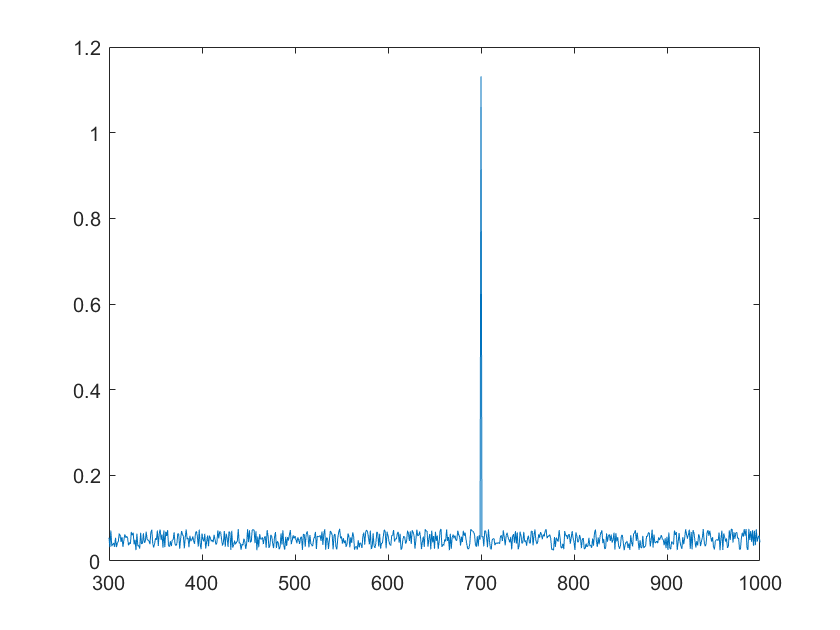
\includegraphics[width=\textwidth]{figures/fig/inter1nm_input.png}

        \label{fig:fig1}
    \end{minipage}
    \hfill
    \begin{minipage}[b]{0.48\textwidth}
        \centering
        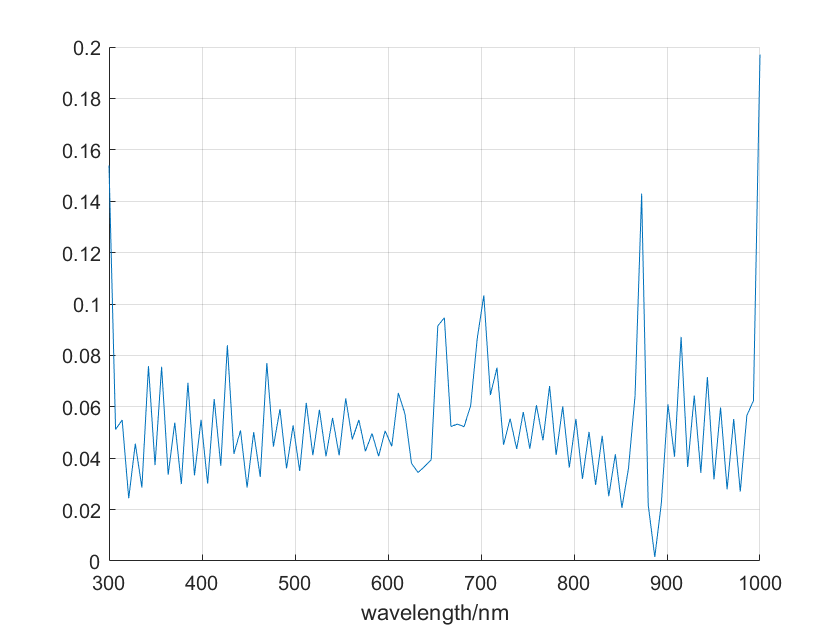
\includegraphics[width=\textwidth]{figures/fig/inter1nm_output.png}

        \label{fig:fig2}
    \end{minipage}

    \caption{1nm间隔采样的响应函数重建效果}
    \label{fig:comparison}
\end{figure}

% 第二组图片
\begin{figure}[H]
    \centering
    \begin{minipage}[b]{0.48\textwidth}
        \centering
        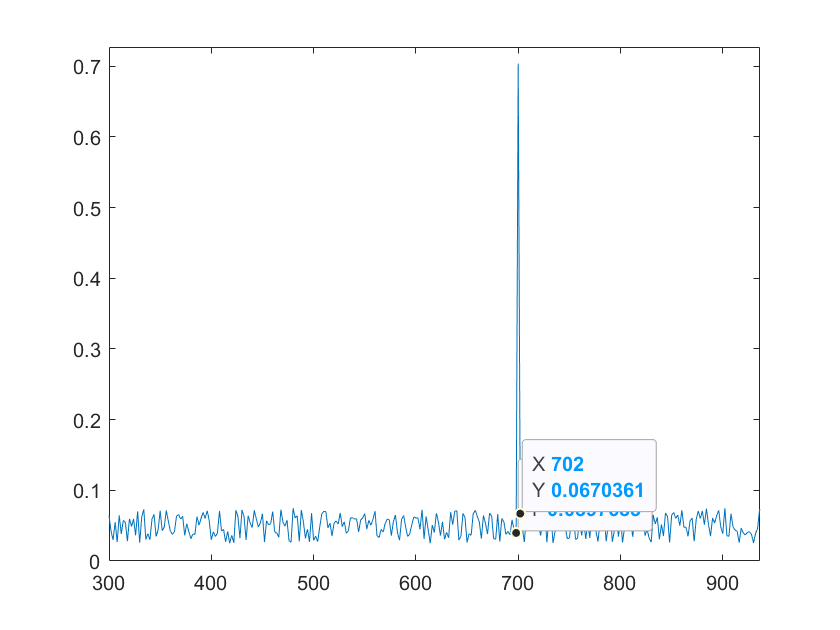
\includegraphics[width=\textwidth]{figures/fig/inter2nm_input.png}

        \label{fig:fig3}
    \end{minipage}
    \hfill
    \begin{minipage}[b]{0.48\textwidth}
        \centering
        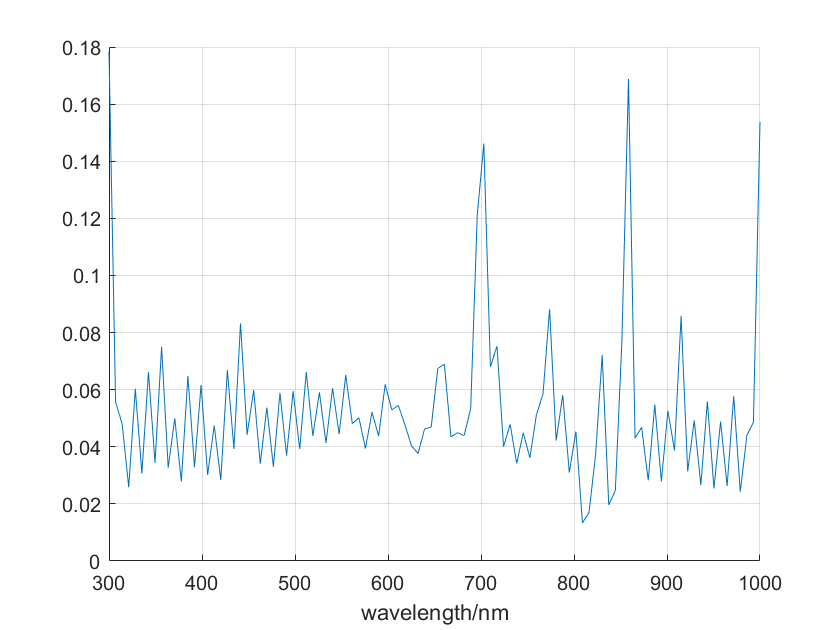
\includegraphics[width=\textwidth]{figures/fig/inter2nm_output.png}

        \label{fig:fig4}
    \end{minipage}
    \caption{2nm间隔采样的响应函数重建效果}
    \label{fig:comparison2}
\end{figure}

% 第三组图片
\begin{figure}[H]
    \centering
    \begin{minipage}[b]{0.48\textwidth}
        \centering
        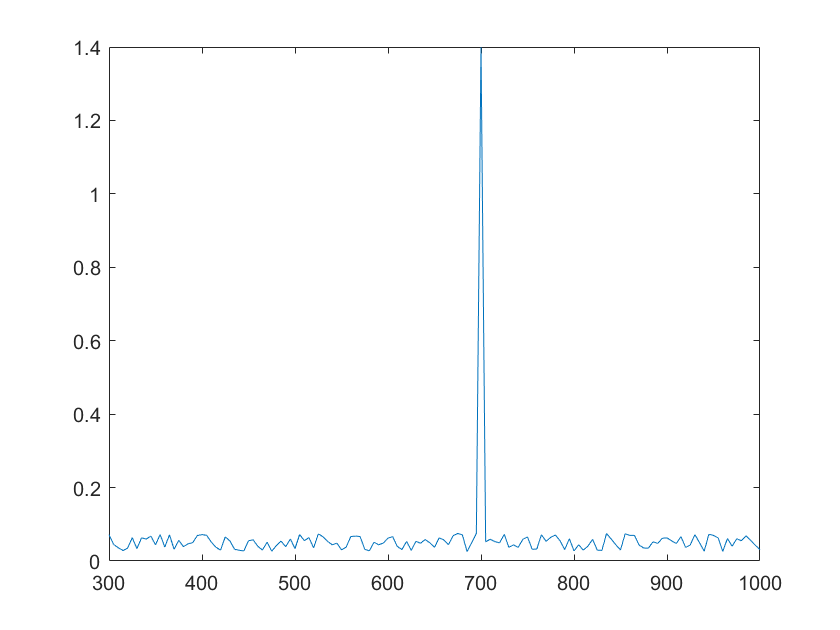
\includegraphics[width=\textwidth]{figures/fig/inter5nm_input.png}

        \label{fig:fig5}
    \end{minipage}
    \hfill
    \begin{minipage}[b]{0.48\textwidth}
        \centering
        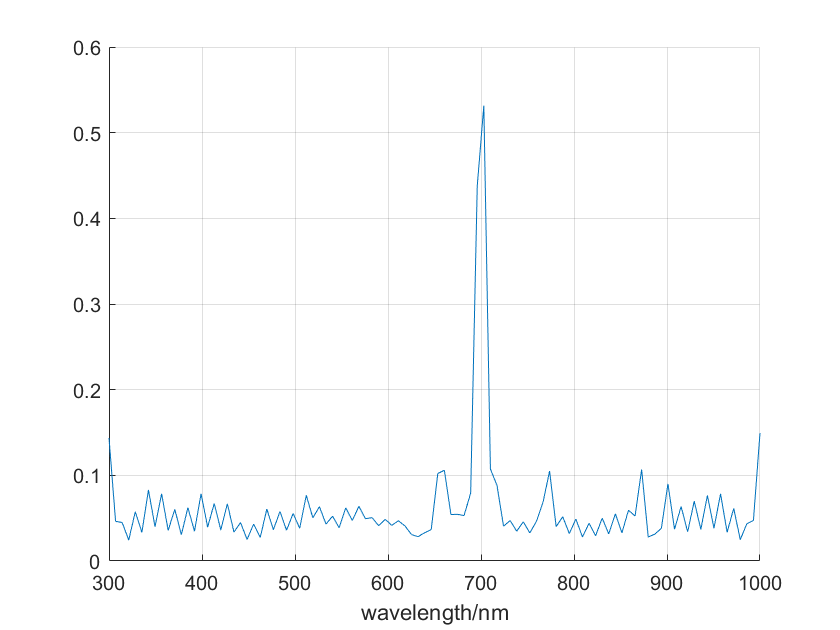
\includegraphics[width=\textwidth]{figures/fig/inter5nm_output.png}

        \label{fig:fig6}
    \end{minipage}
    \caption{5nm间隔采样的响应函数重建效果}
    \label{fig:comparison3}
\end{figure}

% 第四组图片
\begin{figure}[H]
    \centering
    \begin{minipage}[b]{0.48\textwidth}
        \centering
        \includegraphics[width=\textwidth]{figures/fig/inter10nm_input.png}

        \label{fig:fig7}
    \end{minipage}
    \hfill
    \begin{minipage}[b]{0.48\textwidth}
        \centering
        \includegraphics[width=\textwidth]{figures/fig/inter10nm_output.png}

        \label{fig:fig8}
    \end{minipage}
    \caption{10nm间隔采样的响应函数重建效果}
    \label{fig:comparison4}
\end{figure}

% 第五组图片
\begin{figure}[H]
    \centering
    \begin{minipage}[b]{0.48\textwidth}
        \centering
        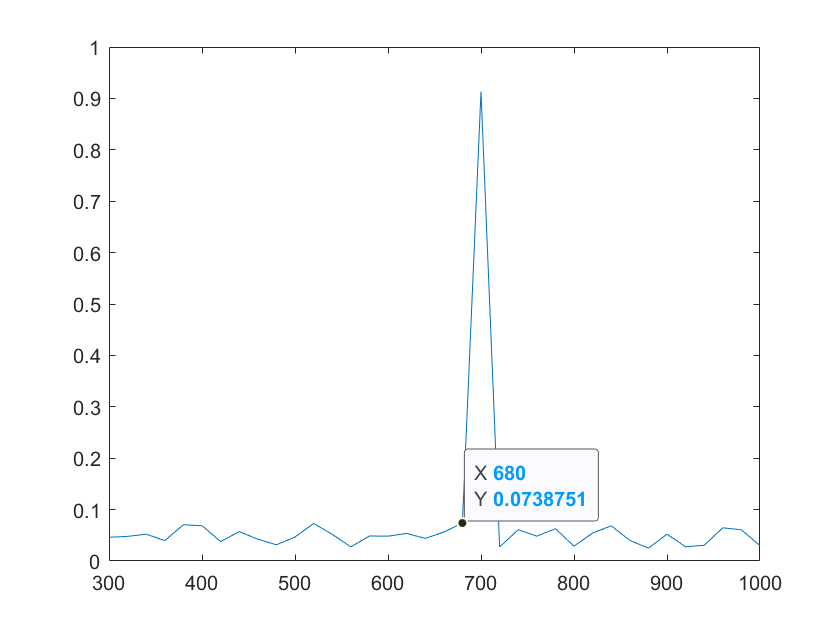
\includegraphics[width=\textwidth]{figures/fig/inter20nm_input.png}

        \label{fig:fig9}
    \end{minipage}
    \hfill
    \begin{minipage}[b]{0.48\textwidth}
        \centering
        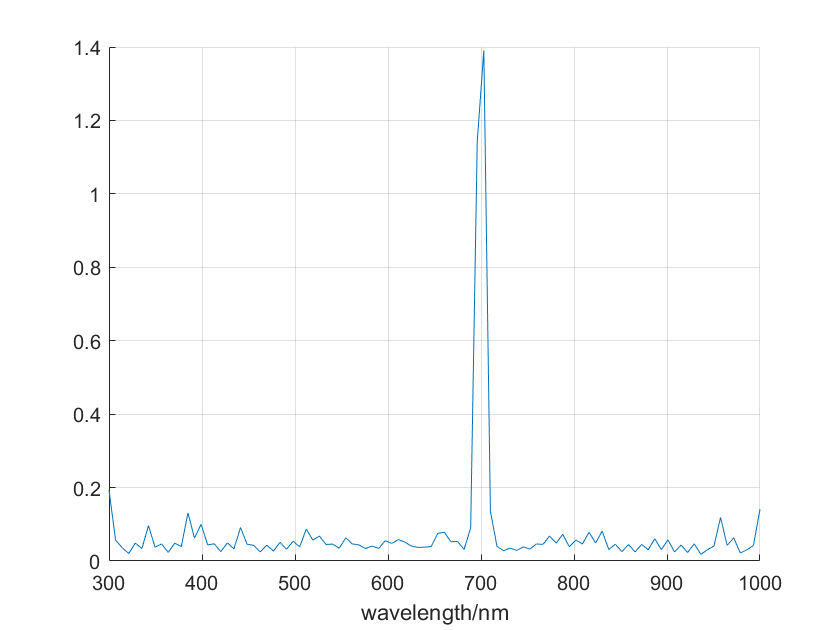
\includegraphics[width=\textwidth]{figures/fig/inter20nm_output.png}

        \label{fig:fig10}
    \end{minipage}
    \caption{20nm间隔采样的响应函数重建效果}
    \label{fig:comparison5}
\end{figure}

通过对比不同间隔采样的响应函数重建效果，我们可以观察到以下几点：
\begin{itemize}
    \item 当采样间隔较小时（如1nm和2nm），重建光谱效果很差，几乎无法重建出输入光谱的特征。
    \item 随着采样间隔的增大（如5nm、10nm和20nm），输入光谱分辨率下降，但是重建光谱的效果逐渐改善，能够较好地反映输入光谱的特征。
\end{itemize}
\textbf{结果分析：}这表明，超表面响应函数的采样间隔对光谱重建的精度有显著影响。较小的采样间隔能够提供更高的分辨率，但是更容易受到噪声的影响，导致重建效果不佳。而较大的采样间隔虽然降低了分辨率，但能够更稳定地重建光谱特征。
其原因可能与超表面的响应函数特性有关，较小的采样间隔可能导致响应函数的高频成分过于复杂，
难以通过简单的重建算法进行有效重建。同时，当采样间隔较小时，需要的传感器通道数量也会显著增加，
但是我们仿真得到的超表面响应函数只有25组,因此无法满足高分辨率采样的需求。导致高分辨率的情况下重建效果不佳。



\subsubsection{单峰光谱重建结果与分析}

\subsubsection*{单峰分辨率极限测试}
为了测试我们的超表面和光谱重建的极限性能，我们采用1nm间隔采样的响应函数对高分辨率的单峰光谱进行重建实验。
首先我们不添加噪声，输入的单峰光谱参数为：中心波长为700 nm，不同宽度的单峰光谱来测试光谱重建的极限性能。
得到的重建结果如下：

\begin{figure}[H]
    \centering
    % 第一组图片
    \begin{minipage}[b]{0.48\textwidth}
        \centering
        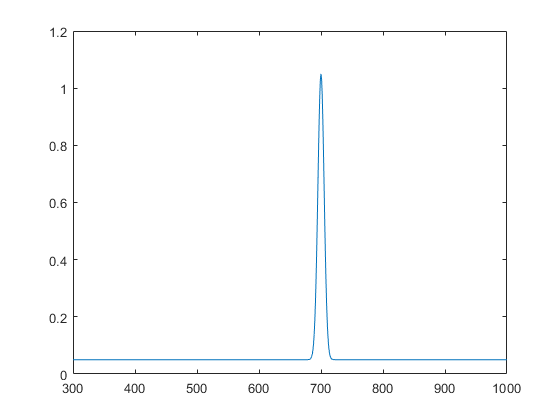
\includegraphics[width=\textwidth]{figures/fig/single40nmwide_input.png}

        \label{fig:fig1}
    \end{minipage}
    \hfill
    \begin{minipage}[b]{0.48\textwidth}
        \centering
        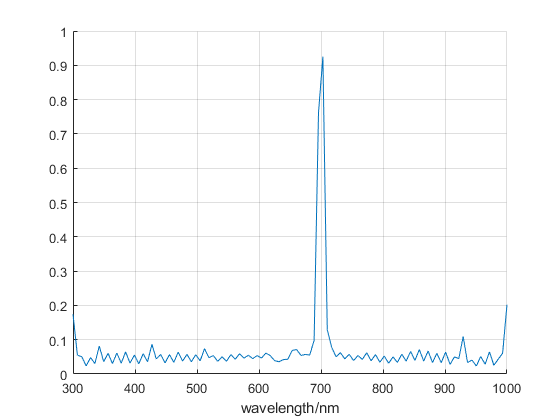
\includegraphics[width=\textwidth]{figures/fig/single40nmwide_output.png}

        \label{fig:fig2}
    \end{minipage}

    \caption{40nm宽度单峰光谱重建效果}
    \label{fig:comparison}
\end{figure}

\begin{figure}[H]
    \centering
    \begin{minipage}[b]{0.48\textwidth}
        \centering
        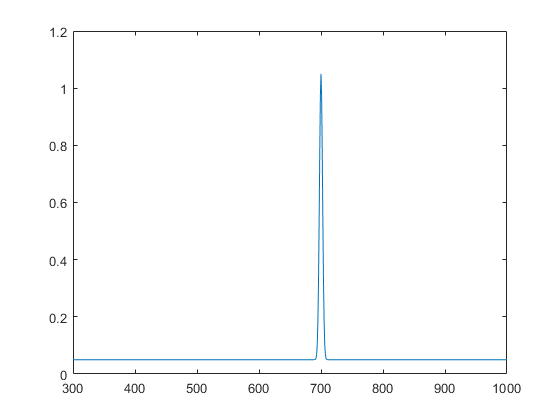
\includegraphics[width=\textwidth]{figures/fig/single20nmwide_input.png}

        \label{fig:fig1}
    \end{minipage}
    \hfill
    \begin{minipage}[b]{0.48\textwidth}
        \centering
        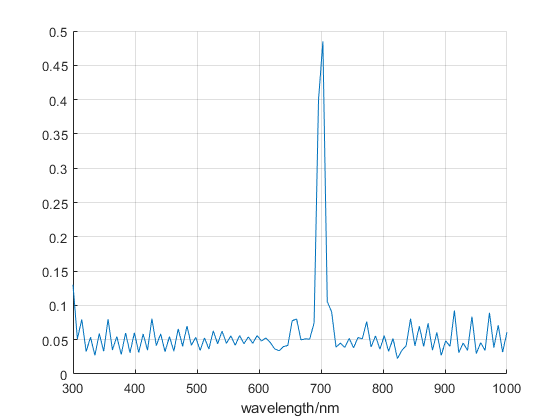
\includegraphics[width=\textwidth]{figures/fig/single20nmwide_output.png}

        \label{fig:fig2}
    \end{minipage}

    \caption{20nm宽度单峰光谱重建效果}
    \label{fig:comparison}
\end{figure}


\begin{figure}[H]
    \centering
    \begin{minipage}[b]{0.48\textwidth}
        \centering
        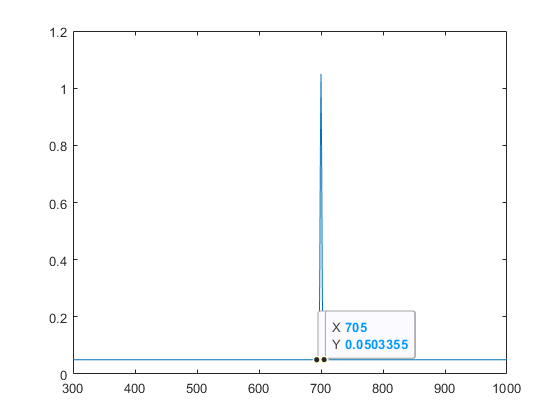
\includegraphics[width=\textwidth]{figures/fig/single12nmwide_input.png}

        \label{fig:fig1}
    \end{minipage}
    \hfill
    \begin{minipage}[b]{0.48\textwidth}
        \centering
        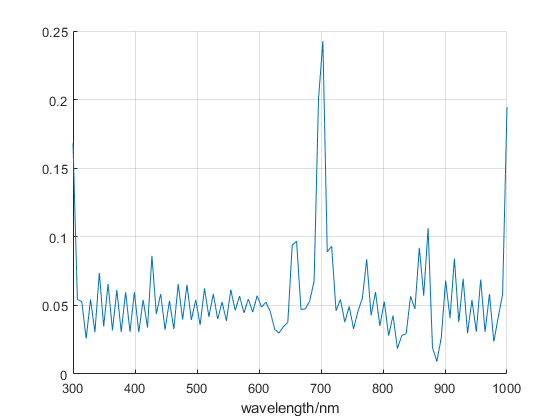
\includegraphics[width=\textwidth]{figures/fig/single12nmwide_outputpng.png}

        \label{fig:fig2}
    \end{minipage}

    \caption{12nm宽度单峰光谱重建效果}
    \label{fig:comparison}
\end{figure}

\begin{figure}[H]
    \centering
    \begin{minipage}[b]{0.48\textwidth}
        \centering
        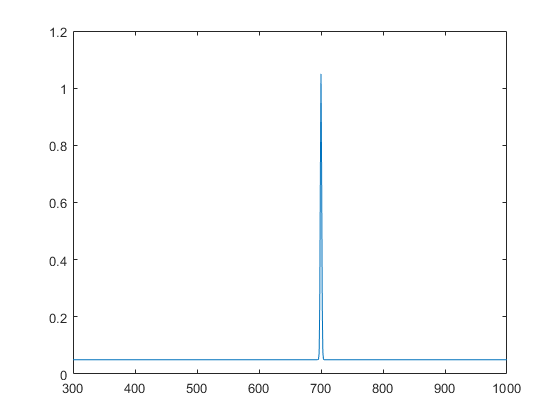
\includegraphics[width=\textwidth]{figures/fig/single10nmwide_input.png}

        \label{fig:fig1}
    \end{minipage}
    \hfill
    \begin{minipage}[b]{0.48\textwidth}
        \centering
        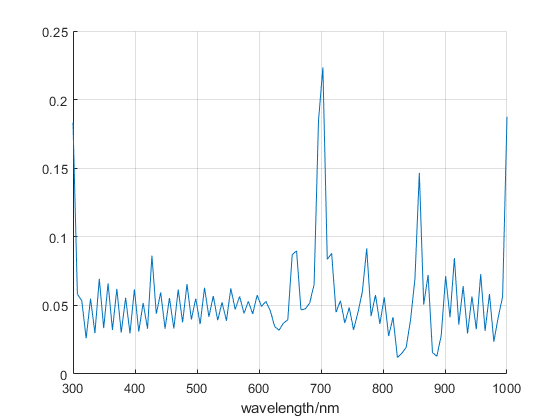
\includegraphics[width=\textwidth]{figures/fig/single10nmwide_output.png}

        \label{fig:fig2}
    \end{minipage}

    \caption{10nm宽度单峰光谱重建效果}
    \label{fig:comparison}
\end{figure}


\begin{figure}[H]
    \centering
    \begin{minipage}[b]{0.48\textwidth}
        \centering
        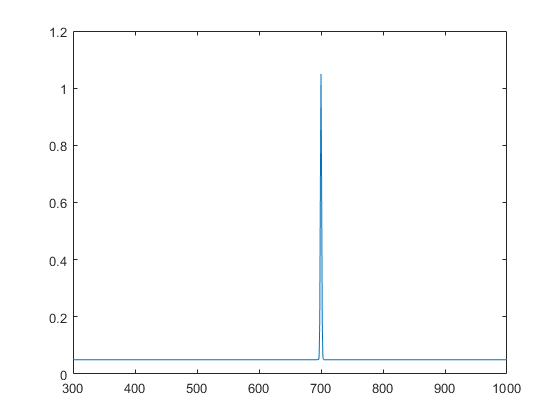
\includegraphics[width=\textwidth]{figures/fig/single8nmwide_input.png}

        \label{fig:fig1}
    \end{minipage}
    \hfill
    \begin{minipage}[b]{0.48\textwidth}
        \centering
        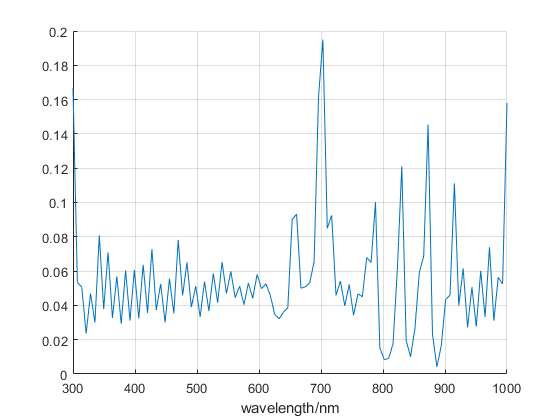
\includegraphics[width=\textwidth]{figures/fig/single8nmwide_output.png}

        \label{fig:fig2}
    \end{minipage}

    \caption{8nm宽度单峰光谱重建效果}
    \label{fig:comparison}
\end{figure}


\begin{figure}[H]
    \centering
    \begin{minipage}[b]{0.48\textwidth}
        \centering
        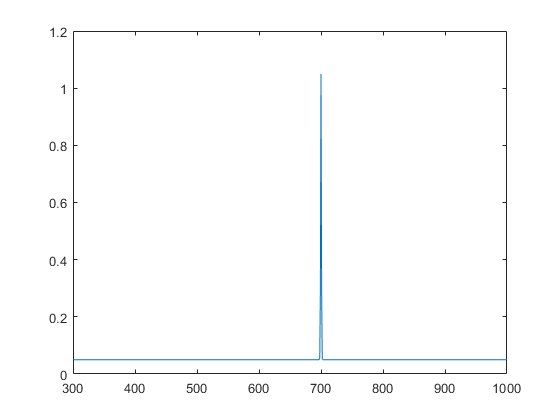
\includegraphics[width=\textwidth]{figures/fig/single6nmwide_input.png}

        \label{fig:fig1}
    \end{minipage}
    \hfill
    \begin{minipage}[b]{0.48\textwidth}
        \centering
        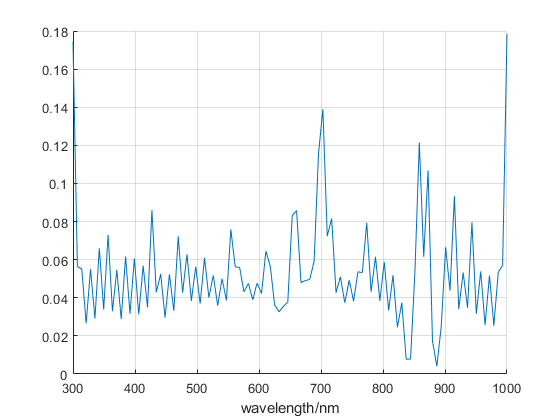
\includegraphics[width=\textwidth]{figures/fig/single6nmwide_output.png}

        \label{fig:fig2}
    \end{minipage}

    \caption{6nm宽度单峰光谱重建效果}
    \label{fig:comparison}
\end{figure}

通过对比不同宽度的单峰光谱重建效果，我们可以观察到以下几点：
\begin{itemize}
    \item 当单峰光谱宽度较大时（如40nm和20nm），重建效果较好，能够较准确地反映输入光谱的特征。
    \item 随着单峰光谱宽度的减小（如12nm、10nm、8nm），重建效果逐渐下降，尤其是当宽度小于等于8nm时，重建结果开始出现明显的偏差。
    \item 当单峰光谱宽度等于6nm时，重建效果非常差，几乎无法重建出输入光谱的特征。达到了超表面和光谱重建的极限性能。
\end{itemize}

\textbf{结果分析：}
可见，在不添加噪声的情况下，超表面和光谱重建算法能够较好地重建宽度较大的单峰光谱，但对于宽度较小的单峰光谱，重建效果明显下降。
这表明，超表面和光谱重建算法对于单峰光的极限分辨率在6nm左右，超过这个分辨率后，重建效果会显著下降，无法准确重建出输入光谱的特征。


\subsubsection*{抗噪声极限测试}

接下来，我们测试光谱重建的抗噪声极限。采用 1nm 间隔采样的响应函
数，设置输入的单峰光谱参数为：中心波长为700 nm，宽度12nm.设置不同的噪声强度
得到的重建结果如下：

\begin{figure}[H]
    \centering
    \begin{minipage}[b]{0.48\textwidth}
        \centering
        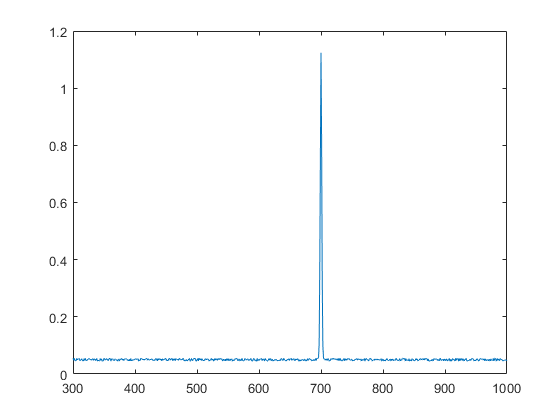
\includegraphics[width=\textwidth]{figures/fig/single_0.1noise.png}

        \label{fig:fig1}
    \end{minipage}
    \hfill
    \begin{minipage}[b]{0.48\textwidth}
        \centering
        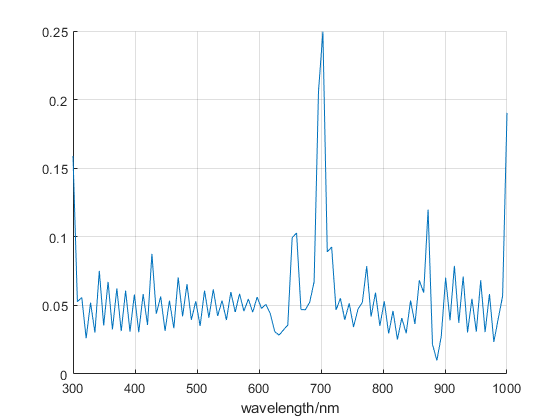
\includegraphics[width=\textwidth]{figures/fig/single_0.1noise_out.png}

        \label{fig:fig2}
    \end{minipage}

    \caption{噪声强度为0.1的单峰光谱重建效果}
    \label{fig:comparison}
\end{figure}

\begin{figure}[H]
    \centering
    \begin{minipage}[b]{0.48\textwidth}
        \centering
        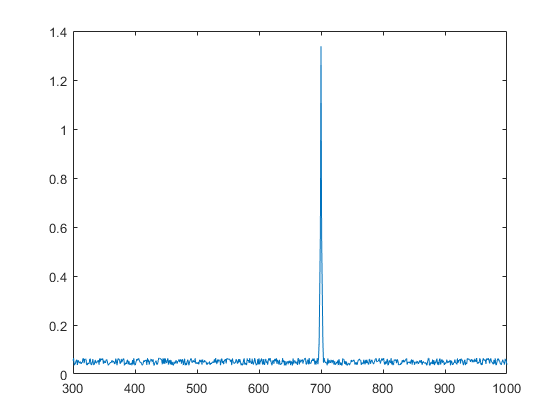
\includegraphics[width=\textwidth]{figures/fig/single_0.3noise.png}

        \label{fig:fig1}
    \end{minipage}
    \hfill
    \begin{minipage}[b]{0.48\textwidth}
        \centering
        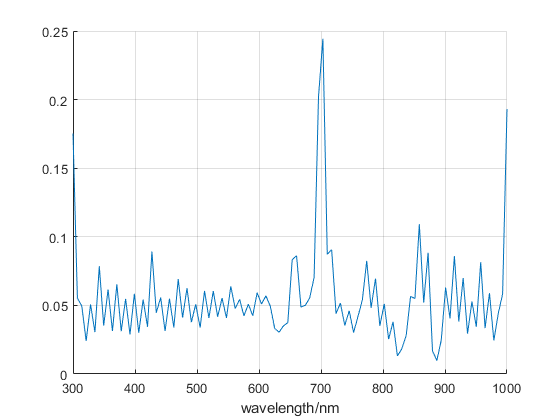
\includegraphics[width=\textwidth]{figures/fig/single_0.3noise_out.png}

        \label{fig:fig2}
    \end{minipage}

    \caption{噪声强度为0.3的单峰光谱重建效果}
    \label{fig:comparison}
\end{figure}


\begin{figure}[H]
    \centering
    \begin{minipage}[b]{0.48\textwidth}
        \centering
        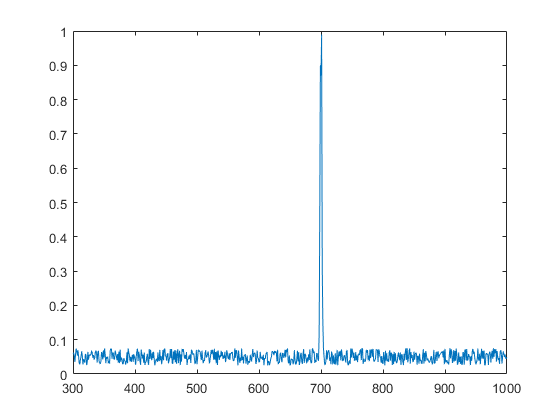
\includegraphics[width=\textwidth]{figures/fig/single_0.5noise.png}

        \label{fig:fig1}
    \end{minipage}
    \hfill
    \begin{minipage}[b]{0.48\textwidth}
        \centering
        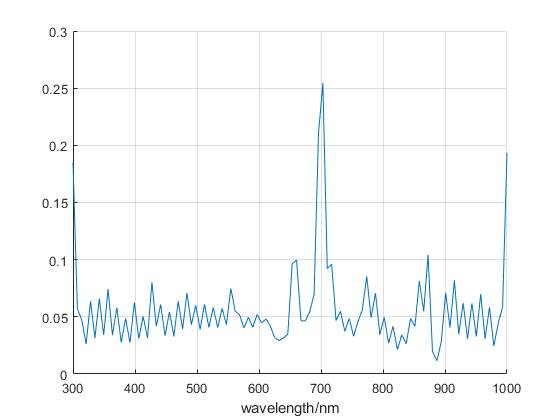
\includegraphics[width=\textwidth]{figures/fig/single_0.5noise_out.png}

        \label{fig:fig2}
    \end{minipage}

    \caption{噪声强度为0.5的单峰光谱重建效果}
    \label{fig:comparison}
\end{figure}



\begin{figure}[H]
    \centering
    \begin{minipage}[b]{0.48\textwidth}
        \centering
        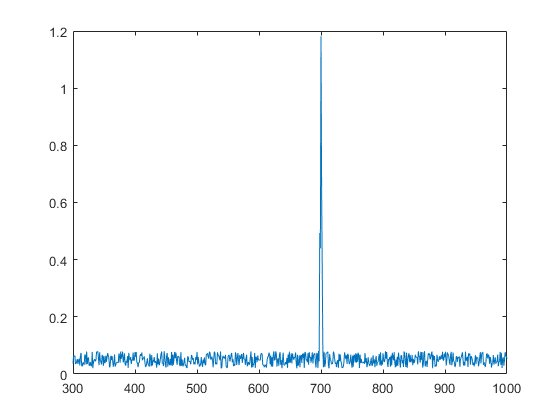
\includegraphics[width=\textwidth]{figures/fig/single_0.6noise.png}

        \label{fig:fig1}
    \end{minipage}
    \hfill
    \begin{minipage}[b]{0.48\textwidth}
        \centering
        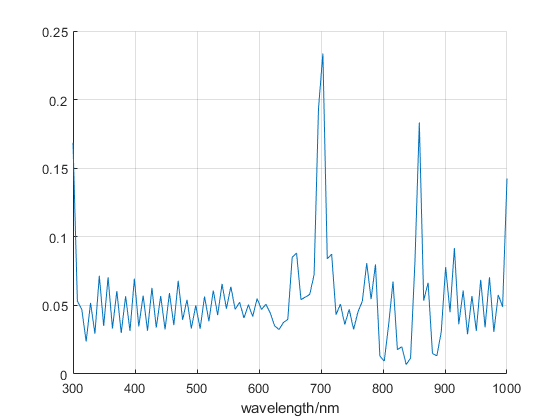
\includegraphics[width=\textwidth]{figures/fig/single_0.6noise_out.png}

        \label{fig:fig2}
    \end{minipage}

    \caption{噪声强度为0.6的单峰光谱重建效果}
    \label{fig:comparison}
\end{figure}


\begin{figure}[H]
    \centering
    \begin{minipage}[b]{0.48\textwidth}
        \centering
        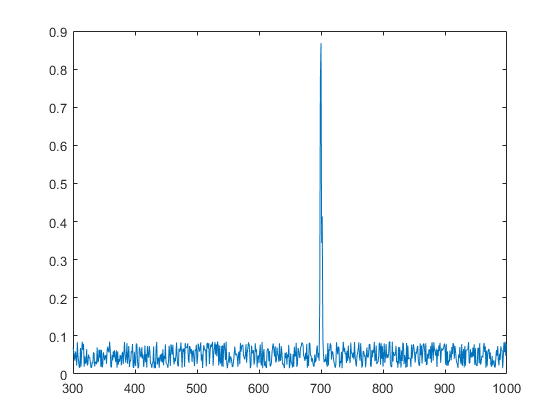
\includegraphics[width=\textwidth]{figures/fig/single_0.7noise.png}

        \label{fig:fig1}
    \end{minipage}
    \hfill
    \begin{minipage}[b]{0.48\textwidth}
        \centering
        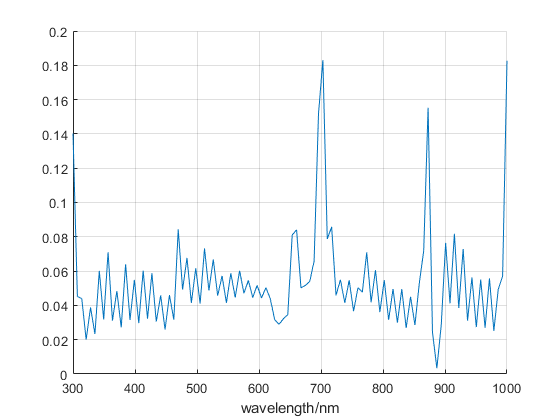
\includegraphics[width=\textwidth]{figures/fig/single_0.7noise_out.png}

        \label{fig:fig2}
    \end{minipage}

    \caption{噪声强度为0.7的单峰光谱重建效果}
    \label{fig:comparison}
\end{figure}

\begin{figure}[H]
    \centering
    \begin{minipage}[b]{0.48\textwidth}
        \centering
        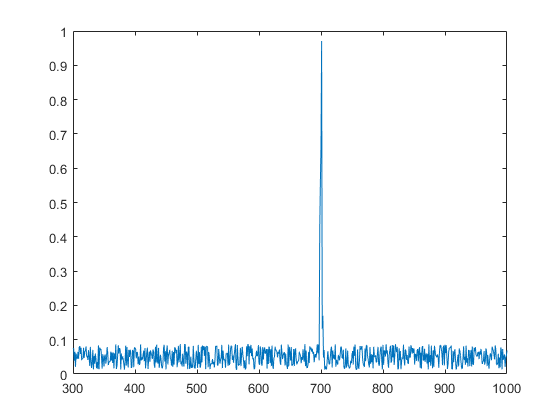
\includegraphics[width=\textwidth]{figures/fig/single_0.75noise.png}

        \label{fig:fig1}
    \end{minipage}
    \hfill
    \begin{minipage}[b]{0.48\textwidth}
        \centering
        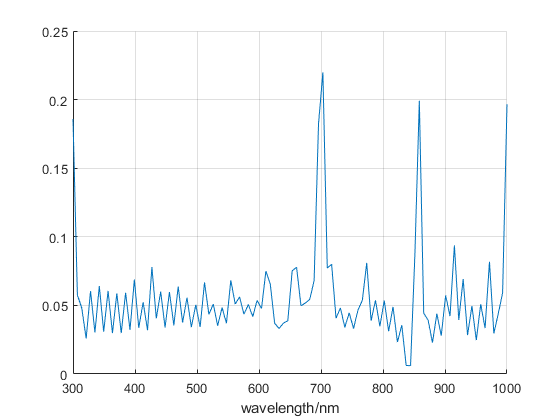
\includegraphics[width=\textwidth]{figures/fig/single_0.75noise_out.png}

        \label{fig:fig2}
    \end{minipage}

    \caption{噪声强度为0.75的单峰光谱重建效果}
    \label{fig:comparison}
\end{figure}

\textbf{结果分析：}
   随着噪声强度的增加，重建效果逐渐下降。当噪声强度较低（如 0.1 或 0.3）时，重建光谱能够较好地反映输入光谱的特征，重建误差较小，说明算法在低噪声环境下具有较强的鲁棒性。然而，当噪声强度逐渐增大（如 0.5 或 0.6）时，重建光谱开始出现明显的偏差，尤其是在光谱的峰值位置和宽度上，重建结果与输入光谱的差异逐渐增大。

   对于我们设置的输入单峰光谱参数（中心波长为 700 nm，宽度为 12 nm），当噪声强度达到 0.7 至 0.75 时，重建效果明显下降，无法准确重建出输入光谱的特征。此时，重建光谱的峰值位置偏移，宽度也发生了显著变化，甚至出现了无法辨识的重建结果。这表明，光谱重建算法的抗噪声极限约为 0.7。

   在噪声强度较高的情况下，噪声对光谱的峰值和宽度特征造成了严重破坏，导致重建光谱无法准确反映输入光谱的真实形态。这种现象可能与噪声对测量矩阵的扰动有关，噪声的增加会降低测量矩阵的稀疏性，从而影响重建算法的性能。

\subsubsection{双峰光谱重建结果与分析}

\subsubsection*{双峰分辨率极限测试}

我们采用 1nm 间隔采样的响应函
数对高分辨率的双峰光谱进行重建实验。首先我们不添加噪声，输入
单个峰宽度为12nm,不同间距的的双峰光谱来测试光谱重建的极限性能。得到的重建结
果如下：


\begin{figure}[H]
    \centering
    \begin{minipage}[b]{0.48\textwidth}
        \centering
        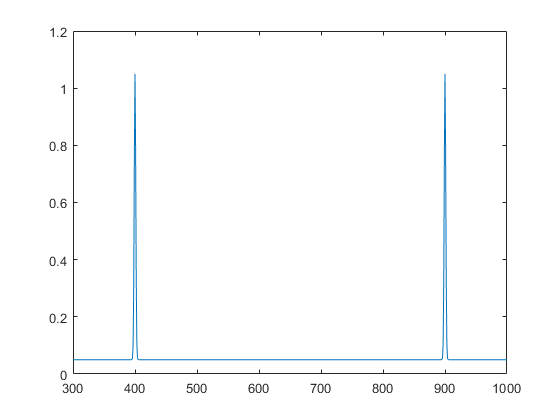
\includegraphics[width=\textwidth]{figures/fig/dual_501_3001.png}

        \label{fig:fig1}
    \end{minipage}
    \hfill
    \begin{minipage}[b]{0.48\textwidth}
        \centering
        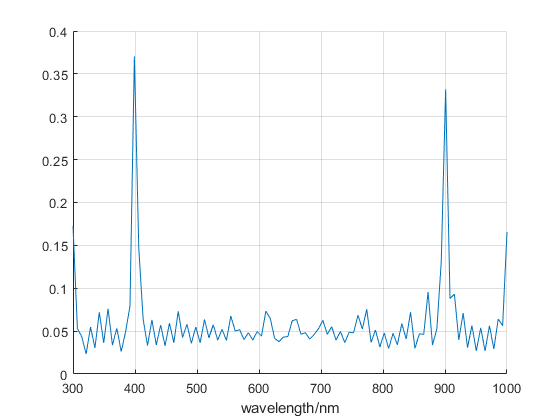
\includegraphics[width=\textwidth]{figures/fig/dual_501_3001_out.png}

        \label{fig:fig2}
    \end{minipage}

    \caption{间距为500nm的双峰光谱重建效果}
    \label{fig:comparison}
\end{figure}


\begin{figure}[H]
    \centering
    \begin{minipage}[b]{0.48\textwidth}
        \centering
        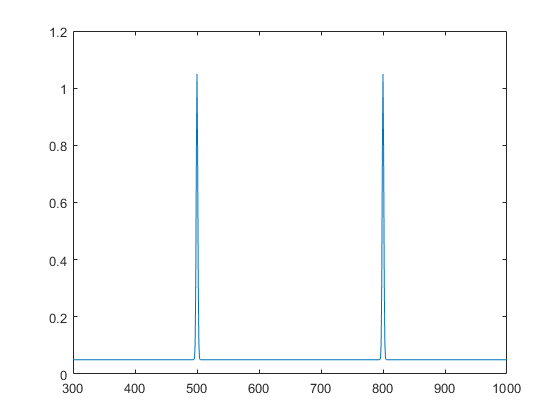
\includegraphics[width=\textwidth]{figures/fig/dual_1001_2501.png}

        \label{fig:fig1}
    \end{minipage}
    \hfill
    \begin{minipage}[b]{0.48\textwidth}
        \centering
        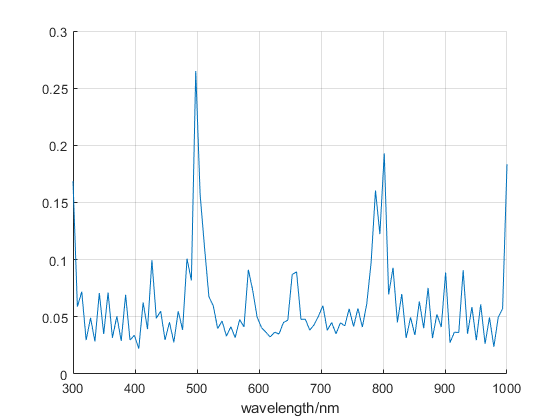
\includegraphics[width=\textwidth]{figures/fig/dual_1001_2501_out.png}

        \label{fig:fig2}
    \end{minipage}

    \caption{间距为300nm的双峰光谱重建效果}
    \label{fig:comparison}
\end{figure}

\begin{figure}[H]
    \centering
    \begin{minipage}[b]{0.48\textwidth}
        \centering
        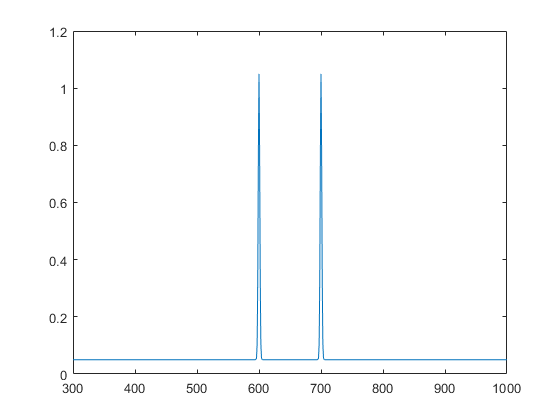
\includegraphics[width=\textwidth]{figures/fig/dual_1501_2001.png}

        \label{fig:fig1}
    \end{minipage}
    \hfill
    \begin{minipage}[b]{0.48\textwidth}
        \centering
        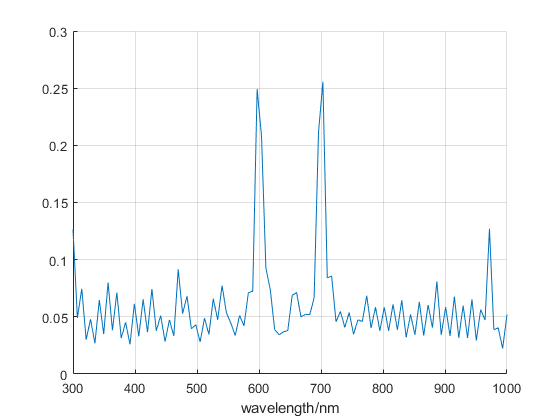
\includegraphics[width=\textwidth]{figures/fig/dual_1501_2001_out.png}

        \label{fig:fig2}
    \end{minipage}

    \caption{间距为100nm的双峰光谱重建效果}
    \label{fig:comparison}
\end{figure}


\begin{figure}[H]
    \centering
    \begin{minipage}[b]{0.48\textwidth}
        \centering
        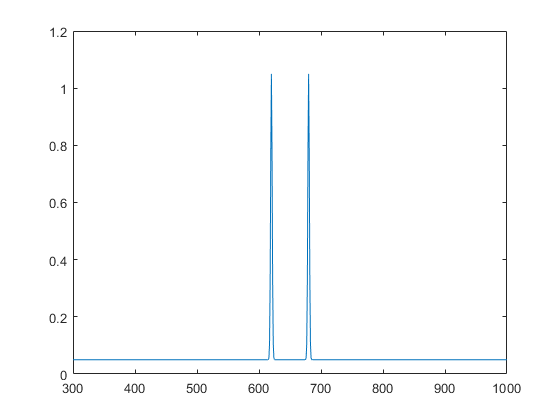
\includegraphics[width=\textwidth]{figures/fig/dual_1601_1901.png}

        \label{fig:fig1}
    \end{minipage}
    \hfill
    \begin{minipage}[b]{0.48\textwidth}
        \centering
        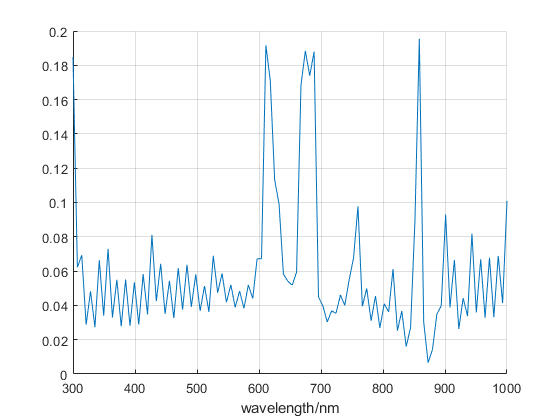
\includegraphics[width=\textwidth]{figures/fig/dual_1601_1901_out.png}

        \label{fig:fig2}
    \end{minipage}

    \caption{间距为60nm的双峰光谱重建效果}
    \label{fig:comparison}
\end{figure}




\begin{figure}[H]
    \centering
    \begin{minipage}[b]{0.48\textwidth}
        \centering
        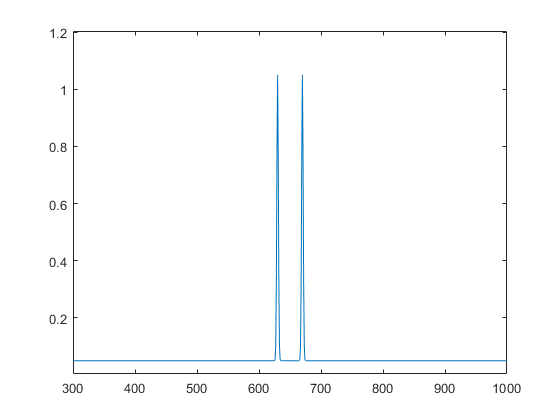
\includegraphics[width=\textwidth]{figures/fig/dual_1651_1851.png}

        \label{fig:fig1}
    \end{minipage}
    \hfill
    \begin{minipage}[b]{0.48\textwidth}
        \centering
        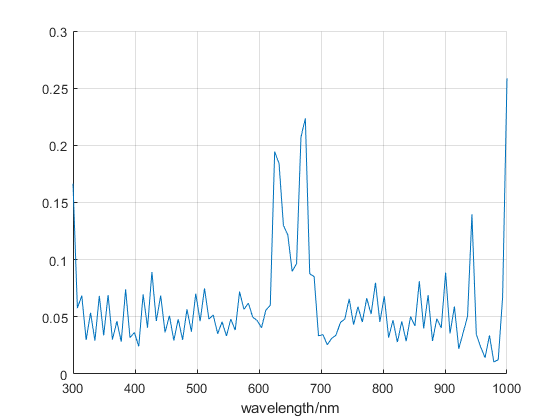
\includegraphics[width=\textwidth]{figures/fig/dual_1651_1851_out.png}

        \label{fig:fig2}
    \end{minipage}

    \caption{间距为40nm的双峰光谱重建效果}
    \label{fig:comparison}
\end{figure}

\begin{figure}[H]
    \centering
    \begin{minipage}[b]{0.48\textwidth}
        \centering
        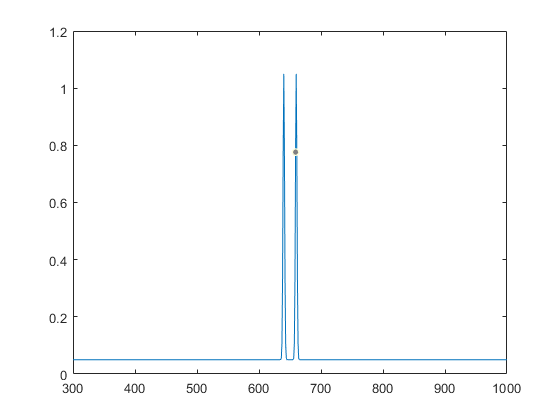
\includegraphics[width=\textwidth]{figures/fig/dual_1701_1801.png}

        \label{fig:fig1}
    \end{minipage}
    \hfill
    \begin{minipage}[b]{0.48\textwidth}
        \centering
        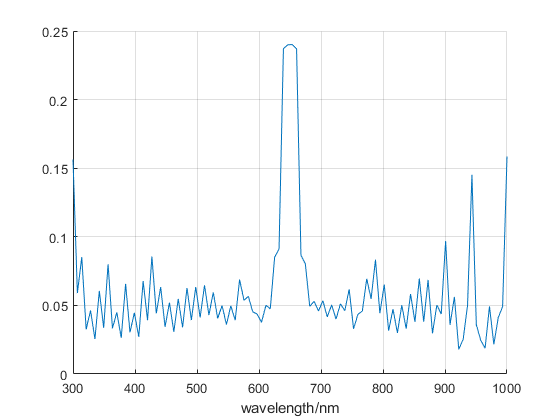
\includegraphics[width=\textwidth]{figures/fig/dual_1701_1801_out.png}

        \label{fig:fig2}
    \end{minipage}

    \caption{间距为20nm的双峰光谱重建效果}
    \label{fig:comparison}
\end{figure}

\textbf{结果分析：}  
通过对不同间距的双峰光谱重建效果进行对比，可以得出以下结论：  
 
当双峰光谱的间距较大时（如 500 nm 和 300 nm），重建效果较好，两个峰的峰值位置和宽度能够较准确地反映输入光谱的特征，说明算法在处理宽间距双峰光谱时具有较强的鲁棒性。然而，随着双峰间距的逐渐减小（如 100 nm 和 60 nm），重建效果开始下降，两个峰的分离度降低，甚至出现峰值融合的现象。

当双峰间距进一步减小到 20 nm 时，重建效果显著下降，两个峰几乎无法分辨，重建光谱呈现出单峰的形态。这表明，光谱重建算法的双峰分辨率极限约为 40 nm。当间距小于该值时，算法无法有效区分两个峰的特征。
从图中可见，分辨双缝的极限间距大约在40nm左右


在实际应用中，为了保证双峰光谱的重建精度，需要综合考虑光谱间距和超表面响应函数的分辨率。对于间距较小的双峰光谱，可以通过优化超表面设计或采用更高分辨率的测量矩阵来提高重建效果。此外，结合更先进的重建算法（如深度学习方法）可能进一步提升分辨率极限。

综上所述，光谱重建算法在处理宽间距双峰光谱时表现出较好的鲁棒性，但其分辨率极限约为 40 nm。当双峰间距小于该值时，重建效果显著下降，无法准确区分两个峰的特征。这一结果为超表面设计和光谱重建算法的优化提供了重要参考。

\subsubsection*{抗噪声极限测试}
接下来，我们使用100nm间距的双峰光谱进行重建实验，设置不同的噪声强度来测试光谱重建的抗噪声极限。结果如下：

\begin{figure}[H]
    \centering
    \begin{minipage}[b]{0.48\textwidth}
        \centering
        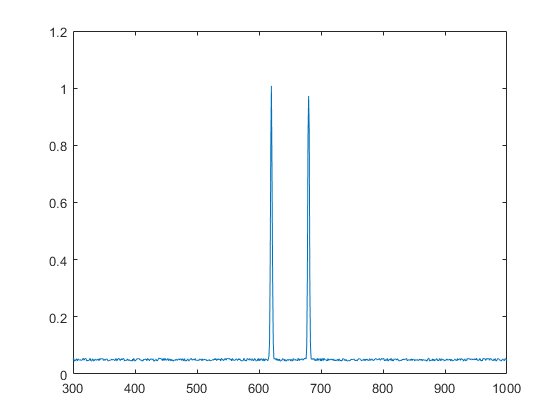
\includegraphics[width=\textwidth]{figures/fig/dual_0.1noise.png}

        \label{fig:fig1}
    \end{minipage}
    \hfill
    \begin{minipage}[b]{0.48\textwidth}
        \centering
        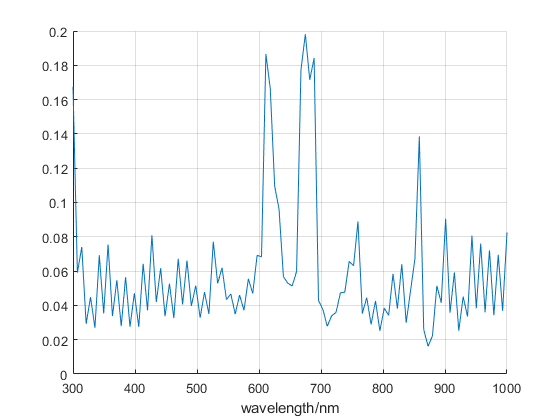
\includegraphics[width=\textwidth]{figures/fig/dual_0.1noise_out.png}

        \label{fig:fig2}
    \end{minipage}

    \caption{噪声强度为0.1的双峰光谱重建效果}
    \label{fig:comparison}
\end{figure}

\begin{figure}[H]
    \centering
    \begin{minipage}[b]{0.48\textwidth}
        \centering
        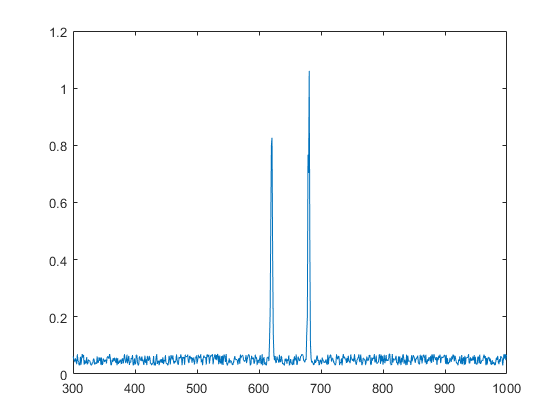
\includegraphics[width=\textwidth]{figures/fig/dual_0.4noise.png}

        \label{fig:fig1}
    \end{minipage}
    \hfill
    \begin{minipage}[b]{0.48\textwidth}
        \centering
        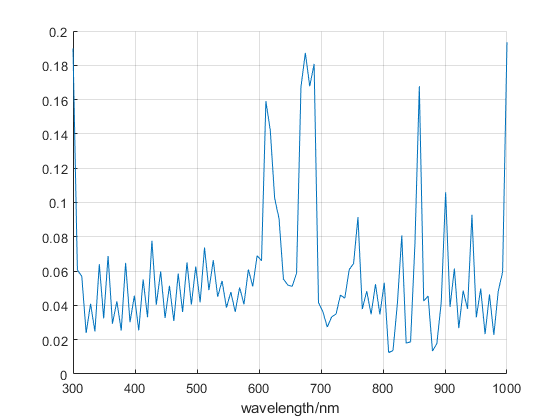
\includegraphics[width=\textwidth]{figures/fig/dual_0.4noise_out.png}

        \label{fig:fig2}
    \end{minipage}

    \caption{噪声强度为0.4的双峰光谱重建效果}
    \label{fig:comparison}
\end{figure}

\begin{figure}[H]
    \centering
    \begin{minipage}[b]{0.48\textwidth}
        \centering
        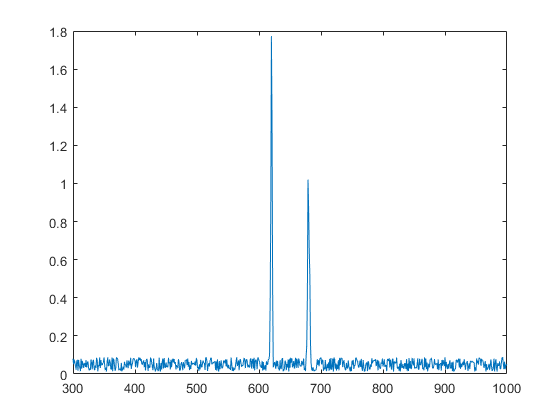
\includegraphics[width=\textwidth]{figures/fig/dual_0.75noise.png}

        \label{fig:fig1}
    \end{minipage}
    \hfill
    \begin{minipage}[b]{0.48\textwidth}
        \centering
        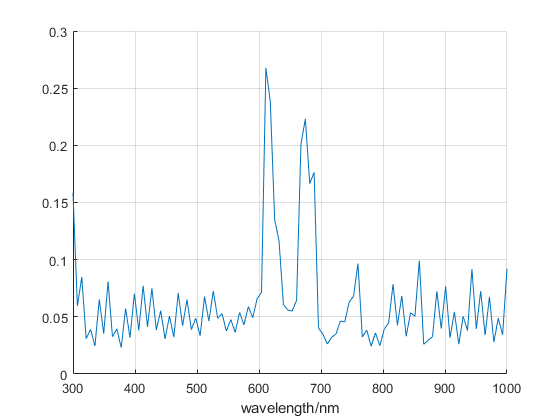
\includegraphics[width=\textwidth]{figures/fig/dual_0.75noise_out.png}

        \label{fig:fig2}
    \end{minipage}

    \caption{噪声强度为0.75的双峰光谱重建效果}
    \label{fig:comparison}
\end{figure}


\begin{figure}[H]
    \centering
    \begin{minipage}[b]{0.48\textwidth}
        \centering
        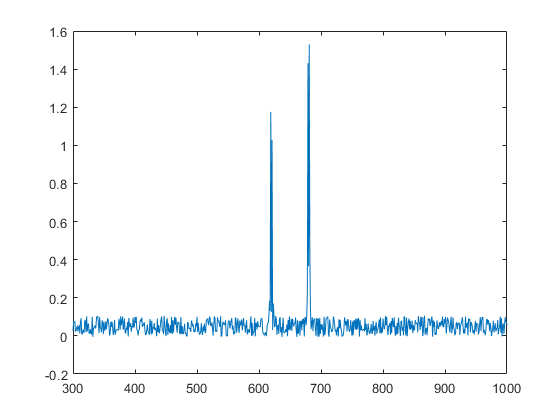
\includegraphics[width=\textwidth]{figures/fig/dual_1.1noise.png}

        \label{fig:fig1}
    \end{minipage}
    \hfill
    \begin{minipage}[b]{0.48\textwidth}
        \centering
        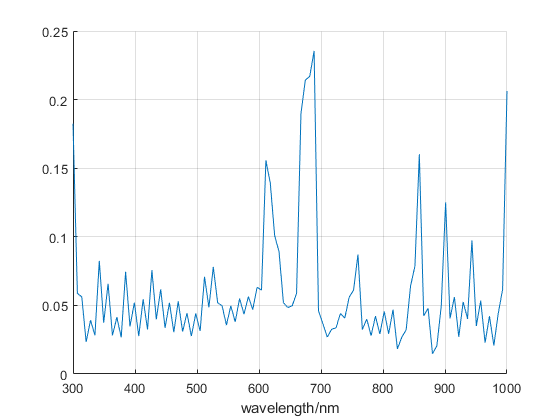
\includegraphics[width=\textwidth]{figures/fig/dual_1.1noise_out.png}

        \label{fig:fig2}
    \end{minipage}

    \caption{噪声强度为1.1的双峰光谱重建效果}
    \label{fig:comparison}
\end{figure}

\begin{figure}[H]
    \centering
    \begin{minipage}[b]{0.48\textwidth}
        \centering
        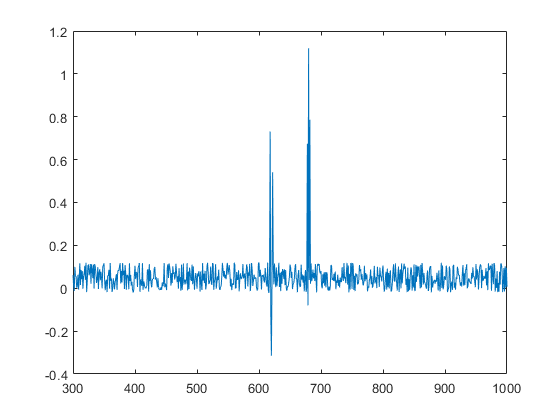
\includegraphics[width=\textwidth]{figures/fig/dual_1.4noise.png}

        \label{fig:fig1}
    \end{minipage}
    \hfill
    \begin{minipage}[b]{0.48\textwidth}
        \centering
        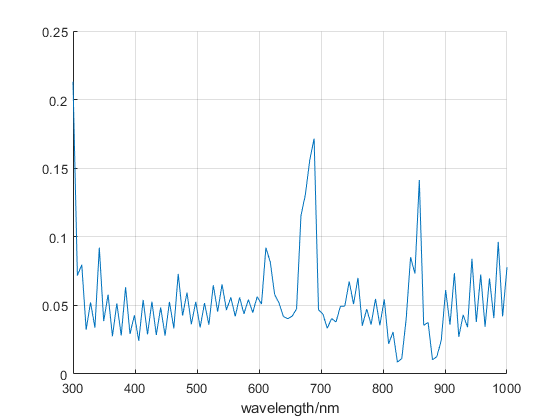
\includegraphics[width=\textwidth]{figures/fig/dual_1.4noise_out.png}

        \label{fig:fig2}
    \end{minipage}

    \caption{噪声强度为1.4的双峰光谱重建效果}
    \label{fig:comparison}
\end{figure}

\textbf{结果分析：}
可以看出，双峰光谱对于噪声的抗性较强。当噪声强度较低（如 0.1 或 0.4,0.7）时，重建光谱能够较好地反映输入光谱的特征，说明算法在低噪声环境下具有较强的鲁棒性。
直到噪声强度非常大以至于破坏原有双峰光谱的特征时（如 1.1 或 1.4），重建效果开始显著下降，两个峰的分离度降低，甚至出现峰值融合的现象。

\subsubsection{宽光谱重建结果与分析}
我们测试了宽光谱的重建效果，使用1nm间隔采样的响应函数，输入宽光谱进行测试。
重建效果如下：
\begin{figure}[H]
    \centering
    \begin{minipage}[b]{0.48\textwidth}
        \centering
        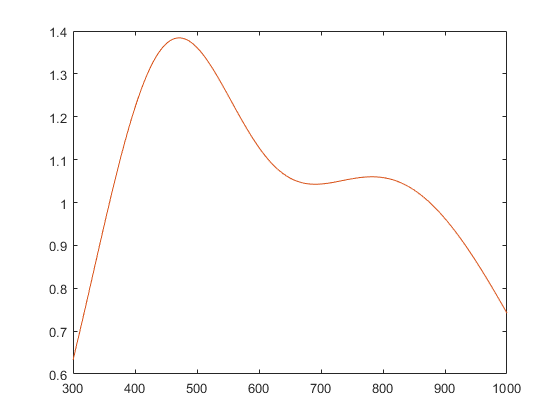
\includegraphics[width=\textwidth]{figures/fig/wide_input.png}

        \label{fig:fig1}
    \end{minipage}
    \hfill
    \begin{minipage}[b]{0.48\textwidth}
        \centering
        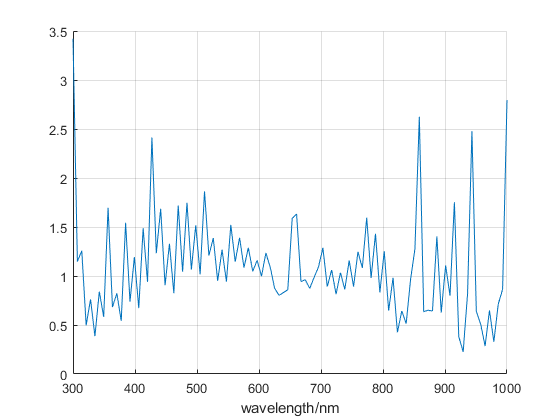
\includegraphics[width=\textwidth]{figures/fig/wide_output.png}

        \label{fig:fig2}
    \end{minipage}

    \caption{宽光谱重建效果}
    \label{fig:comparison}
\end{figure}
我们测试了各种采样间隔的响应函数和不同参数的宽光谱重建效果，最终发现
重建效果均不佳，无法准确重建出输入光谱的特征。

\textbf{结果分析：}造成这种现象的原因可能是宽光谱的频率成分较多，
导致重建算法难以有效捕捉到光谱的特征，且响应函数数量太少，
实际获得的光谱信息不足以支撑宽光谱的重建。


\section{总结}

本文围绕基于超表面的光谱重建技术展开了深入研究，主要内容和结论如下：

\subsection*{1. 超表面设计与仿真}
通过对超表面结构的设计与仿真，我们成功构建了25组不同响应函数的超表面。仿真结果表明，超表面能够通过调整光栅的厚度、宽度、周期和材料等参数，实现对不同波长光的高效调控。这为后续的光谱重建提供了可靠的测量矩阵。

\subsection*{2. 光谱重建算法}
基于高斯基展开的正则化方法，我们实现了从压缩信号到光谱分布的重建。实验表明，该方法能够在低噪声环境下有效抑制噪声并提高重建精度。同时，通过广义交叉验证（GCV）自动选择正则化参数，确保算法在不同场景下的适应性。

\subsection*{3. 光谱重建实验与分析}
我们设计了多组光谱重建实验，分析了不同参数对重建效果的影响：
\begin{itemize}
    \item \textbf{采样间隔的影响}：较大的采样间隔（如10nm和20nm）能够稳定重建光谱特征，但分辨率较低；较小的采样间隔（如1nm和2nm）虽然分辨率较高，但重建效果容易受到噪声影响。
    \item \textbf{单峰光谱分辨率极限}：实验表明，超表面和光谱重建算法的单峰分辨率极限约为6nm。当单峰宽度小于该值时，重建效果显著下降。
    \item \textbf{双峰光谱分辨率极限}：双峰光谱的分辨率极限约为40nm。当双峰间距小于该值时，重建算法无法有效区分两个峰的特征。
    \item \textbf{抗噪声性能}：在噪声强度较低（如0.1或0.3）时，重建效果较好；当噪声强度超过0.7时，重建效果显著下降，无法准确反映输入光谱的特征。
    \item \textbf{宽光谱重建}：由于宽光谱的频率成分复杂且响应函数数量有限，重建效果不佳，无法准确捕捉光谱特征。
\end{itemize}

\subsection*{4. 研究意义与展望}
本研究通过结合超表面设计与光谱重建算法，验证了基于超表面的光谱重建技术的可行性和局限性。研究结果表明：
\begin{itemize}
    \item 超表面在光谱调控和压缩感知采样方面具有显著优势，为光谱成像技术的紧凑化和高效化提供了新思路。
    \item 光谱重建算法在低噪声环境下表现出较好的鲁棒性，但在高噪声环境和复杂光谱条件下仍需进一步优化。
    \item 当前超表面响应函数的数量和分辨率限制了光谱重建的性能，未来可以通过优化超表面设计或结合深度学习等先进算法进一步提升重建效果。
\end{itemize}

综上所述，基于超表面的光谱重建技术在生物医学、环境监测和工业检测等领域具有广阔的应用前景。未来的研究可以进一步探索超表面设计与重建算法的协同优化，以实现更高分辨率、更强鲁棒性的光谱重建系统。



%%----------- 参考文献 -------------------%%
%在reference.bib文件中填写参考文献，此处自动生成
\newpage
\bibliographystyle{ieeetr}
\bibliography{reference}


\end{document}